\chapter{格林函数法}
\intro{本章深入讨论格林函数的构造、性质和应用。}

\begin{mydefinition}{格林函数}
$G(\vect{x},\vect{\xi})$ 满足：
\[
\begin{cases}
\lapl_{\vect{x}}G(\vect{x},\vect{\xi})=\delta(\vect{x}-\vect{\xi}),&\vect{x}\in\Omega\\
G(\vect{x},\vect{\xi})=0,&\vect{x}\in\partial\Omega
\end{cases}
\]
\end{mydefinition}

\section{格林函数的性质}

\begin{theorem}[对称性]
$G(\vect{x},\vect{\xi})=G(\vect{\xi},\vect{x})$
\end{theorem}

\begin{theorem}[奇异性]
$\displaystyle G(\vect{x},\vect{\xi})\sim-\frac{1}{4\pi|\vect{x}-\vect{\xi}|}$（$\vect{x}\to\vect{\xi}$）
\end{theorem}

\section{典型区域的格林函数}

\begin{mydefinition}{半空间的格林函数（镜像法）}
\[
G(\vect{x},\vect{\xi})=\frac{1}{4\pi}\left(\frac{1}{|\vect{x}-\vect{\xi}|}-\frac{1}{|\vect{x}-\vect{\xi}^*|}\right)
\]
$\vect{\xi}^*$ 为 $\vect{\xi}$ 关于边界的镜像。
\end{mydefinition}

\begin{figure}[htbp]
\centering
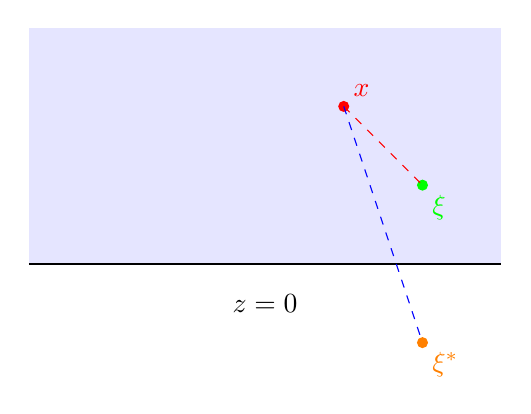
\begin{tikzpicture}
\fill[blue!10] (-3,0) -- (3,0) -- (3,3) -- (-3,3) -- cycle;
\draw[thick] (-3,0) -- (3,0);
\node at (0,-0.5) {$z=0$};
\fill[red] (1,2) circle (2pt) node[above right]{$\vect{x}$};
\fill[green] (2,1) circle (2pt) node[below right]{$\vect{\xi}$};
\fill[orange] (2,-1) circle (2pt) node[below right]{$\vect{\xi}^*$};
\draw[dashed,red] (1,2) -- (2,1);
\draw[dashed,blue] (1,2) -- (2,-1);
\end{tikzpicture}
\caption{镜像法}
\end{figure}

\section{泊松方程的解}

\begin{theorem}[泊松公式]
Dirichlet 问题的解：
\[
u(\vect{x})=\oiint_{\partial\Omega}G(\vect{x},\vect{\xi})\frac{\partial u}{\partial n}\,dS_\xi-\oiint_{\partial\Omega}u(\vect{\xi})\frac{\partial G}{\partial n_\xi}\,dS_\xi+\iiint_\Omega G(\vect{x},\vect{\xi})f(\vect{\xi})\,dV_\xi
\]
\end{theorem}

\begin{remark}
格林函数法将 PDE 求解转化为积分计算。优点是得到显式表达式；缺点是复杂区域的格林函数难以构造。
\end{remark}
